%----------------------------------------------------------------------------------------
%	PACKAGES AND OTHER DOCUMENT CONFIGURATIONS
%----------------------------------------------------------------------------------------

\documentclass{article}

%%%%%%%%%%%%%%%%%%%%%%%%%%%%%%%%%%%%%%%%%
% Lachaise Assignment
% Structure Specification File
% Version 1.0 (26/6/2018)
%
% This template originates from:
% http://www.LaTeXTemplates.com
%
% Authors:
% Marion Lachaise & François Févotte
% Vel (vel@LaTeXTemplates.com)
%
% License:
% CC BY-NC-SA 3.0 (http://creativecommons.org/licenses/by-nc-sa/3.0/)
% 
%%%%%%%%%%%%%%%%%%%%%%%%%%%%%%%%%%%%%%%%%

%----------------------------------------------------------------------------------------
%	PACKAGES AND OTHER DOCUMENT CONFIGURATIONS
%----------------------------------------------------------------------------------------

\usepackage{amsmath,amsfonts,stmaryrd,amssymb} % Math packages
\usepackage[UTF8]{ctex}
\usepackage[colorlinks,linkcolor=blue]{hyperref}

\usepackage{enumerate} % Custom item numbers for enumerations

\usepackage[ruled]{algorithm2e} % Algorithms

\usepackage[framemethod=tikz]{mdframed} % Allows defining custom boxed/framed environments

\usepackage{listings} % File listings, with syntax highlighting
\lstset{
	basicstyle=\ttfamily, % Typeset listings in monospace font
	tabsize=2
}

\usepackage{float} % 图片位置

%----------------------------------------------------------------------------------------
%	DOCUMENT MARGINS
%----------------------------------------------------------------------------------------

\usepackage{geometry} % Required for adjusting page dimensions and margins

\geometry{
	paper=a4paper, % Paper size, change to letterpaper for US letter size
	top=2.5cm, % Top margin
	bottom=3cm, % Bottom margin
	left=2.5cm, % Left margin
	right=2.5cm, % Right margin
	headheight=14pt, % Header height
	footskip=1.5cm, % Space from the bottom margin to the baseline of the footer
	headsep=1.2cm, % Space from the top margin to the baseline of the header
	%showframe, % Uncomment to show how the type block is set on the page
}

%----------------------------------------------------------------------------------------
%	FONTS
%----------------------------------------------------------------------------------------

\usepackage[utf8]{inputenc} % Required for inputting international characters
\usepackage[T1]{fontenc} % Output font encoding for international characters

\usepackage{XCharter} % Use the XCharter fonts

%----------------------------------------------------------------------------------------
%	COMMAND LINE ENVIRONMENT
%----------------------------------------------------------------------------------------

% Usage:
% \begin{commandline}
%	\begin{verbatim}
%		$ ls
%		
%		Applications	Desktop	...
%	\end{verbatim}
% \end{commandline}

\mdfdefinestyle{commandline}{
	leftmargin=10pt,
	rightmargin=10pt,
	innerleftmargin=15pt,
	middlelinecolor=black!50!white,
	middlelinewidth=2pt,
	frametitlerule=false,
	backgroundcolor=black!5!white,
	frametitle={Command Line},
	frametitlefont={\normalfont\sffamily\color{white}\hspace{-1em}},
	frametitlebackgroundcolor=black!50!white,
	nobreak,
}

% Define a custom environment for command-line snapshots
\newenvironment{commandline}{
	\medskip
	\begin{mdframed}[style=commandline]
}{
	\end{mdframed}
	\medskip
}

%----------------------------------------------------------------------------------------
%	FILE CONTENTS ENVIRONMENT
%----------------------------------------------------------------------------------------

% Usage:
% \begin{file}[optional filename, defaults to "File"]
%	File contents, for example, with a listings environment
% \end{file}

\mdfdefinestyle{file}{
	innertopmargin=1.6\baselineskip,
	innerbottommargin=0.8\baselineskip,
	topline=false, bottomline=false,
	leftline=false, rightline=false,
	leftmargin=0cm,
	rightmargin=0cm,
	singleextra={%
		\draw[fill=black!10!white](P)++(0,-1.2em)rectangle(P-|O);
		\node[anchor=north west]
		at(P-|O){\ttfamily\mdfilename};
		%
		\def\l{3em}
		\draw(O-|P)++(-\l,0)--++(\l,\l)--(P)--(P-|O)--(O)--cycle;
		\draw(O-|P)++(-\l,0)--++(0,\l)--++(\l,0);
	},
	nobreak,
}

% Define a custom environment for file contents
\newenvironment{file}[1][File]{ % Set the default filename to "File"
	\medskip
	\newcommand{\mdfilename}{#1}
	\begin{mdframed}[style=file]
}{
	\end{mdframed}
	\medskip
}

%----------------------------------------------------------------------------------------
%	NUMBERED QUESTIONS ENVIRONMENT
%----------------------------------------------------------------------------------------

% Usage:
% \begin{question}[optional title]
%	Question contents
% \end{question}

\mdfdefinestyle{question}{
	innertopmargin=1.2\baselineskip,
	innerbottommargin=0.8\baselineskip,
	roundcorner=5pt,
	nobreak,
	singleextra={%
		\draw(P-|O)node[xshift=1em,anchor=west,fill=white,draw,rounded corners=5pt]{%
		Question \theQuestion\questionTitle};
	},
}

\newcounter{Question} % Stores the current question number that gets iterated with each new question

% Define a custom environment for numbered questions
\newenvironment{question}[1][\unskip]{
	\bigskip
	\stepcounter{Question}
	\newcommand{\questionTitle}{~#1}
	\begin{mdframed}[style=question]
}{
	\end{mdframed}
	\medskip
}

%----------------------------------------------------------------------------------------
%	WARNING TEXT ENVIRONMENT
%----------------------------------------------------------------------------------------

% Usage:
% \begin{warn}[optional title, defaults to "Warning:"]
%	Contents
% \end{warn}

\mdfdefinestyle{warning}{
	topline=false, bottomline=false,
	leftline=false, rightline=false,
	nobreak,
	singleextra={%
		\draw(P-|O)++(-0.5em,0)node(tmp1){};
		\draw(P-|O)++(0.5em,0)node(tmp2){};
		\fill[black,rotate around={45:(P-|O)}](tmp1)rectangle(tmp2);
		\node at(P-|O){\color{white}\scriptsize\bf !};
		\draw[very thick](P-|O)++(0,-1em)--(O);%--(O-|P);
	}
}

% Define a custom environment for warning text
\newenvironment{warn}[1][Warning:]{ % Set the default warning to "Warning:"
	\medskip
	\begin{mdframed}[style=warning]
		\noindent{\textbf{#1}}
}{
	\end{mdframed}
}

%----------------------------------------------------------------------------------------
%	INFORMATION ENVIRONMENT
%----------------------------------------------------------------------------------------

% Usage:
% \begin{info}[optional title, defaults to "Info:"]
% 	contents
% 	\end{info}

\mdfdefinestyle{info}{%
	topline=false, bottomline=false,
	leftline=false, rightline=false,
	nobreak,
	singleextra={%
		\fill[black](P-|O)circle[radius=0.4em];
		\node at(P-|O){\color{white}\scriptsize\bf i};
		\draw[very thick](P-|O)++(0,-0.8em)--(O);%--(O-|P);
	}
}

% Define a custom environment for information
\newenvironment{info}[1][Info:]{ % Set the default title to "Info:"
	\medskip
	\begin{mdframed}[style=info]
		\noindent{\textbf{#1}}
}{
	\end{mdframed}
}
 % Include the file specifying the document structure and custom commands

%----------------------------------------------------------------------------------------
%	ASSIGNMENT INFORMATION
%----------------------------------------------------------------------------------------

\title{编译课程项目报告 \\ \large{—— 语法分析器}} % Title of the assignment

\author{靳帅祥\\ \texttt{16307130023@fudan.edu.cn}} % Author name and email address

\date{\today} % University, school and/or department name(s) and a date

\begin{document}

\maketitle % Print the title

\tableofcontents

\newpage

%----------------------------------------------------------------------------------------
%	INTRODUCTION
%----------------------------------------------------------------------------------------

\section{实验目的} % 加上* Unnumbered section

\begin{itemize}
\setlength{\itemsep}{0pt}
\setlength{\parsep}{0pt}
\setlength{\parskip}{0pt}
    \item 学习LALR文法和Bison语法分析生成器的用法
    \item 熟悉PCAT的语法
    \item 使用bison为PCAT编写语法生成器
    \item 利用上述过程构建抽象语法树并输出
\end{itemize}

%----------------------------------------------------------------------------------------
%	概述
%----------------------------------------------------------------------------------------

\section{概述} % Numbered section

语法分析器是PCAT的编译器中非常重要的一部分。通常一个标准的编译器前端需要包含词法分析器、语法分析器、中间代码生成这几个部分,其中语法分析器的主要任务是读入词法单元流、判断输入程序是否匹配程序设计语言的语法规范,并在匹配规范的情况下构建起输入程序的静态结构。语法分析使得编译器的后续阶段看到的输入程序不再是一串字符流或者单词流,而是一个结构整齐、处理方便的数据对象。本实验中构建的是抽象语法树,将传递给后续的中间码生成步骤。

PCAT的语法可以使用LALR文法描述,对于LALR文法,可以采用成熟的语法分析器生成器,输入LALR文法,并生成词文法对应的语法分析器代码。本实验采用Bison来生成语法分析器,输入PCAT语言的BNF文法描述文件,生成语法分析器,并把生成的语法分析器与上一次实验中的词法分析器组合,完成了可以对源代码进行分析,输出抽象语法树的程序。

%------------------------------------------------

\section{实现过程}

\subsection{语法的整理}

\begin{enumerate}
	\item 阅读《PCAT语言参考指南》,整理出ebnf范式
	\item 把ebnf转化为Bison可以接受的bnf语法,主要是闭包、可选项的转化,发现一些重复的部分,重复的部分虽然形式相同,但其语义可能不同,不能随意合并。
		\begin{enumerate}
			\item varDeclType0 \& procedureDeclType0 重复
			\item varDeclIDArray \& fpSectionIDArray 重复
		\end{enumerate}
	\item 将fixed的PCAT语法加入前面整理的bnf语法中,fixed部分的主要作用是消除语法的二义性,使各个运算符号能够正确的被计算
	\item 继续整理bnf-fixed
		\begin{enumerate}
			\item varDeclIDClosure 和 fpSectionIDClosure 合并为 IDClosure
			\item 把可选项后缀由0改成Option
			\item 添加constant
			\item varDeclType0 和 procedureDeclType0 合并为 typenameOption
		\end{enumerate}
\end{enumerate}

	如何转换闭包和可选项将在后面介绍。

\subsection{重写词法分析器}

第一个PJ中的词法分析器已经不适合于这个PJ,所以对其进行重写,对于每个匹配项返回预定义的Token,方便语法分析其进行处理。
	\subsubsection{\%option noyywrap}
	\textbf{yywrap()}这一函数在文件(或输入)的末尾调用。 如果函数的返回值是1,就停止解析。 因此它可以用来解析多个文件。 代码可以写在第三段,这就能够解析多个文件。
	
	由于本次试验只需要解析一个单独的文件,所以可以使用noyywrap在读完单个文件后,直接结束整个解析过程。
	\subsubsection{\%option yylineno}
	Flex提供的计算行数的工具
	\subsubsection{YY\_USER\_ACTION}
	\begin{info} \\
		The YY\_USER\_ACTION macro is "called" before each of your token actions and updates yylloc.
	\end{info}

	使用这个属性来计算每个Token的位置。
	
	为了更方便的在Bison中获取信息,使用了\textbf{\%locations}这个选项提供的\textbf{YYLTYPE}这个结构体,其定义如下:
	\begin{small}
		\begin{lstlisting}[language=C]
		typedef struct YYLTYPE
		{
			int first_line;
			int first_column;
			int last_line;
			int last_column;
		} YYLTYPE;
		\end{lstlisting}
	\end{small}
	
	在Flex使用yylloc来设置对应Token的位置信息,在每次匹配成功之后,调用下面函数
	\begin{small}
		\begin{lstlisting}[language=C]
		void yylexUpdateLocation() {
			yylloc.first_line = yylineno;
			yylloc.last_line = yylineno;
			yylloc.first_column = yycolumn;
			yylloc.last_column = yycolumn + yyleng - 1;
			yycolumn += yyleng;
		}
		\end{lstlisting}
	\end{small}
	
	之后在Bison中就可以使用\textbf{@\$}或者用\textbf{@n}来获取Token的位置信息。

	\subsubsection{test locations}
	由于现在还没有实现Bison部分,所以在助教提供的demo中来测试上述方法是否可以使用。
	
	\begin{figure}[H]
		\centering
		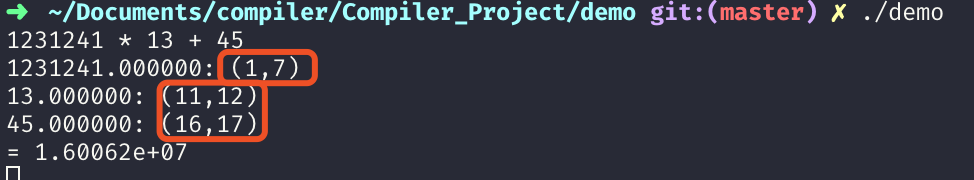
\includegraphics[width=0.7\linewidth]{locationtest}
		\caption{位置信息}
		\label{fig:locationtest}
	\end{figure}

	代码在\textbf{./lextests/demo}中。

	\subsubsection{test scaner}
	在\textbf{./lextests}文件中编写了测试文件来进行测试,测试结果在\textbf{./lextests/out}中。
	
	\begin{commandline}
		\begin{verbatim}
		$ chmod +x lextest.sh
		$ ./lextest.sh
		\end{verbatim}
	\end{commandline}
	
\subsection{语法分析器}

	\subsubsection{Bison介绍}
	Bison是一个GNU系列项⽬中的语法分析器⽣生成工具,它接受⼀个LALR⽂法,并生成一份与之对应的语法分析器源码。Bison接受的LALR文法以BNF范式进行描述,生成语法分析器的代码。
	
	\subsubsection{语法描述文件}
	Bison接受BNF范式描述的LALR文法,描述包含在文法描述文件中。
	
	文件的结构和Flex类似,也是分为三个部分。
	
	\begin{small}
		\begin{lstlisting}
		/*定义部分*/
		%%
		/*规则部分*/
		%%
		/*用户函数部分*/
		\end{lstlisting}
	\end{small}

	\subsubsection{定义部分}
	声明部分主要负责引⽤头⽂文件,设置Bison的参数,定义Token等工作。在文件的顶部可以引用头⽂件,⽬的是允许后续语义动作中调⽤其他源码⽂件中的函数,这一部分使⽤⼀ 对“\%{”与“\%}”符号来标识,其内部可以写入C语言\#include语句、函数或者变量的定义。
	
	此后设置Bison参数,定义Token和非终结符,这类设置通常以“\%”开头。在Bison中,每一个Token或⾮终结符都对应⼀个数据类型,这就允许在进⾏语法分析的过程中,利用每个符号所对应的信息来构造抽象语法树。在此实验中构造语法树的方法也是如此,每⼀个符号都是语法树的⼀个节点,在分析过程中利⽤语义动作来构造语法树。
	
	“\%token”指令⽤用于定义Token及其类型,与词法分析器中输出的Token类型相对应。 
	
	“\%type”指令⽤用于定义⾮非终结符的类型,通常可以定义为抽象语法树的节点。
	
	此外,“\%left”、 “\%right”等指令定义运算符的结合顺序,⽤用于消除冲突。由于修改过的语法已经考虑了运算符号的优先级,所以本次试验中未使用到这些指令。
	
	\subsubsection{规则部分}
	规则部分是整个描述文件中最重要的部分,
	
	规则部分是由BNF语法与语义动作构成的,每一条文法规则都可以使用BNF描述,又可以为规则附加一条语义规则。Bison接受无右递归的非二义性LALR文法。在表达式产生冲突时,可以使用算符优先级解决冲突。
	
	语义动作是当采⽤一条规则归约后就会执⾏的⼀段代码,在这段代码中可以访问所归约语句的所有信息,包括获取终结符与非终结符的值,以及设置产⽣生式左部非终结符的值。在本实验中,所有⾮终结符都保存抽象语法树节点类型的值,在语义动作中,根据不同的语句来构造不同的⼦树。

	\subsubsection{用户函数部分}
	尾部在⽂件中是并不是必要的。有时会希望在语法分析器中写⼊函数等代码,则可以把它们写在这一部分。例如语义动作中调⽤的函数就可以在此处实现;也可以把用到的函数写在其他的C或CPP文件之中,在规则⽂件中仅引用其头文件,在编译时链接后编译成一个完整的可执行文件。
	
%------------------------------------------------

\subsection{PCAT文法的实现}
	在前面{\color{blue}{语法的整理}}部分遗留的两个问题是闭包 和 可选项的ebnf语法转化为bnf语法。
	
	\subsubsection*{闭包的转化}
	闭包是指允许某一个符号重复出现任意次数的形式。需要将其转化为bnf语法,转化规则如下:
	\begin{small}
		\begin{lstlisting}
		ebnf: {A}
		bnf:  AClosure: %empty | AClosure A;
		\end{lstlisting}
	\end{small}
	
	由此引入了一类新的非终结符,他们表示语法树种的一组节点;除此之外,其他的非终结符则表示一个普通的语法树节点。因此,对于任何改写后的闭包(名称后缀种有Closure),都采用了astList类型;对于其他的非终结符,都采用ast类型。

	\subsubsection*{可选项的转化}
	可选项是指一个符号出现1次或者0次。
	\begin{small}
		\begin{lstlisting}
		ebnf: [A]
		bnf:  AOption: %empty | A;
		\end{lstlisting}
	\end{small}	
	
	完成这一部分的整理之后,就完成了一大部分的工作。需要对编写的语法规则进行测试。
	
	
	\subsubsection{正确性测试}
	在测试中,由于还没有编写任何的语义动作,会使用Bison默认的语义动作\{ \$\$ = \$1 \}来进行。
	
	此时,可以将所以得非终结符都设置为相同类型,方便后面的测试。
		
	在调试过程中发现自己编写的语法出现错误,但不知道问题出在哪里,所以需要Bison更加详细的调试信息。下面是几个用到的选项:
	
	\begin{itemize}
		\item \%error-verbose : 可以让报错更加详细
		\subitem
		\begin{small}
			\begin{lstlisting}
*** "syntax error" (line: 5, token:`i')

*** "syntax error, unexpected IDENTIFIER, expecting BEGINT or VAR or TYPE or PROCEDURE" (line: 5, token:`i')
			\end{lstlisting}
		\end{small}
	
		\item -report=state -v 以及 -g : 可以生成关于语法的详细信息。
			\subitem -report=state -v 可以将Bison生成的LALR分析表输出出来
			\subitem -g 可以将整个表输出位一个.dot文件,使用Graphviz软件可以将图像画出来,便于查错
	\end{itemize}
	
	但由于语法很复杂,通过上面的输出并不容易找到错位在哪里,还可以使用Bison提供的debug模式,他会把每一个移进/规约操作都输出出来。开启debug模式的方式是使用-t或者--debug命令,并在主程序中设置把yydebug这个变量设置为1,这是Bison提供的一个变量。
	
	经过调试,发现是自己的语法规则中少写了一条,导致后面的所有语法都无效。
	
	\begin{small}
		\begin{lstlisting}
		andOperand: andOperand AND relationship
		| relationship // 少了这一行
		;
		\end{lstlisting}
	\end{small}
	
	修复这个错误之后就可以判断程序是否符合PCAT的语法,但现在还不能输出语法树。
	
	上述测试在\textbf{./bisontests}文件夹中。
	
	\begin{commandline}
		\begin{verbatim}
		$ chmod +x build.sh
		$ ./build.sh
		\end{verbatim}
	\end{commandline}

	测试结果在\textbf{./bisontests/out}中,19有语法错误,少了一个分号;20是词法错误;其余文件都正确。


\subsection{抽象语法树的实现}
	词法分析器使⽤用⼀个全局变量yylval来传递Token的值,此值是⼀个联合体,在Bison语法规则⽂件的定义部分定义。本实验中定义如下:
	\begin{figure}[H]
		\centering
		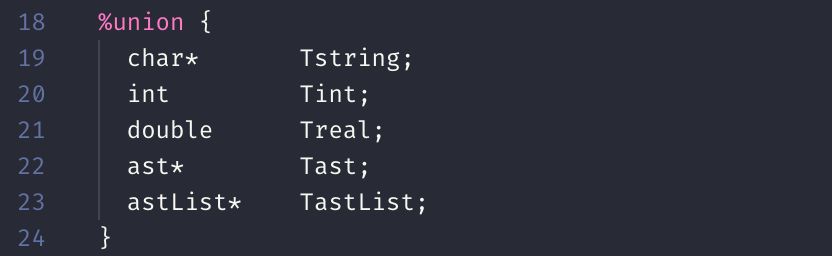
\includegraphics[width=0.7\linewidth]{define}
		\caption{类型定义}
		\label{fig:define}
	\end{figure}

	在以上的定义之下,可以使⽤yylval.Tstring以字符串指针的类型来设置Token值,同理也可以使⽤yylval.Tint以整数类型来设置Token值。在词法分析器的分析动作中,对字符串、整数、实数,以及标识符几种类型的Token添加代码,逐一对yylval赋值。
	
	与Token关联的内容,除了值以外还有源码位置信息。在Bison规则⽂件的声明部分加入\%locations参数,就可以开启词法分析器的位置跟踪。词法分析器中,位置跟踪也是通过一个全局变量yylloc传递给语法分析器的。具体介绍和使用方法见\textbf{3.2.4}。
	
	之后在Bison的语法规则⽂件中就可以引⽤Token的位置了。Bison⽂件的语义动作中,每⼀个终结符或⾮终结符都可以通过“@”符号来引⽤其位置信息。对于终结符,位置信息就是Token的位置,对于非终结符,默认会根据它所包含的第⼀个Token与最后⼀个Token来确定它的位置信息。
	
	抽象语法树的生成是通过语义动作来完成的,对于终结符,其语义动作中利用yylval,调用"ast.h"中定义的语法树相关函数来创建节点。
	\begin{figure}[H]
		\centering
		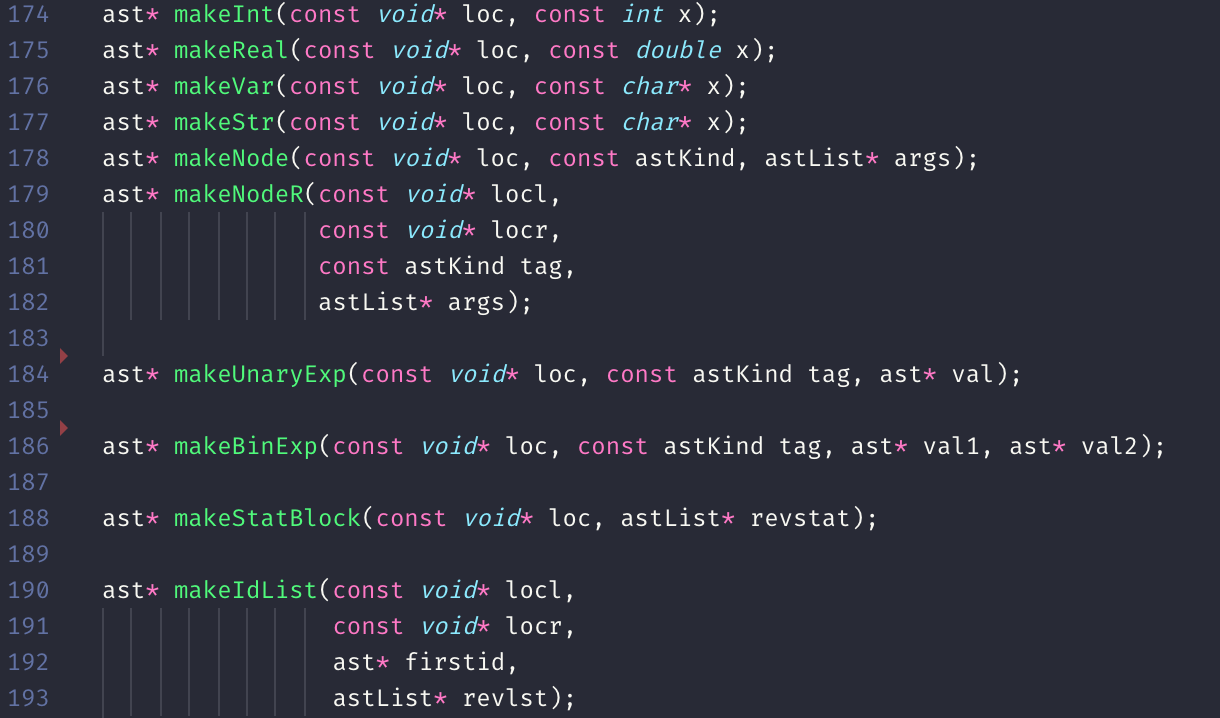
\includegraphics[width=0.7\linewidth]{astdefine}
		\caption{ast相关函数}
		\label{fig:astdefine}
	\end{figure}
	
	对于终结符节点创建,由于只有4种节点,所以直接写成了4个函数,函数接受位置信息和终结符的值,返回一个ast指针类型的树节点。以number为例子来说明如何创建。
		
	语义动作中,"@\$"表⽰归约结果的位置信息,传递给makeInt函数⽤于构造语法树;⽽"\$\$"表⽰归约结果的值,把构造出的语法树赋予归约结果,以便后续分析进一步使用。
	
	除了makeInt函数,"ast.h"中还定义了⼀系列构造语法树的函数。这⼀类函数几乎都接受一个位置信息的指针,用于在构造语法树时保存位置数据。此外,不同的函数接受不同的其他参数。对于终结符,通常需要接受⼀个具体的Token值,例如前⽂提到的整数节点需要接受一个整数值,而对于字符串节点与标识符节点,则需要接受一个字符串值;
	对于⾮终结符,则需要接受一组ast指针类型的语法树节点,例如makeBinExp用于构造⼆元运算表达式。
	
	所有的常规⾮终结符都是ast指针类型的抽象语法树节点。这类节点可以包含具体的值 (如整数、实数、字符串等),或是一颗子树。结构体ast中定义了⼀一个 astTag枚举字段,⽤于唯⼀确定此节点的类型,通过这个类型就可以确定节点是否为⼦树,以及子树的具体结构。对于每一种语法树节点都创建一个枚举值。
	makeInt、makeReal、makeVar、makeStr函数为非终结符创建一个单独的节点,⽽makeNode函数可以创建⼀个通用的子树,还定义了一些函数来简化构造过程。
	
	在拥有抽象语法树后,把树的内容打印出来,就可以十分⽅方便的检验语法分析结果是否正确。在"ast.c"中实现了语法树的打印函数printAst,在文法的开始符号中,创建一个打印整棵语法树的语义动作,就可以在整个代码被接受时打印出来语法树了。
	
	在打印的过程中,根据根据当前节点的位置信息来决定是否换行缩进:如果当前节点与上一节点不在同一⾏行,则换⾏并添加缩进,反之则不换行缩进。
	
	\begin{info}
		
		在编译的过程用遇到了循环引用的问题,在ast.h中引入了pcat.h,在pcat.y中引入了ast.h;在ast.h中引入了pcat.h是为了使用YYLTYPE这个类型,所以定义一个一样的类型来解决循环引用的问题。
		
		在mac下使用clang编译也有一些问题,所以需要使用gcc套件进行编译。
	\end{info}

	\begin{commandline}
		\begin{verbatim}
		$ chmod +x build.sh
		$ ./build.sh
		\end{verbatim}
	\end{commandline}

	输出结果在\textbf{./out}中,对于语法错误,可以输出所在的行号以及期望的符号。
	
	\begin{figure}[H]
		\centering
		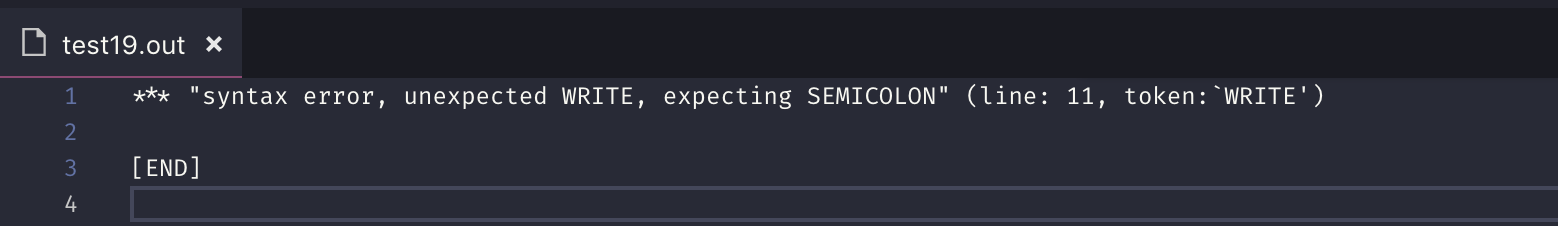
\includegraphics[width=0.7\linewidth]{error}
		\caption{错误提示}
		\label{fig:error}
	\end{figure}

	\begin{figure}[H]
		\centering
		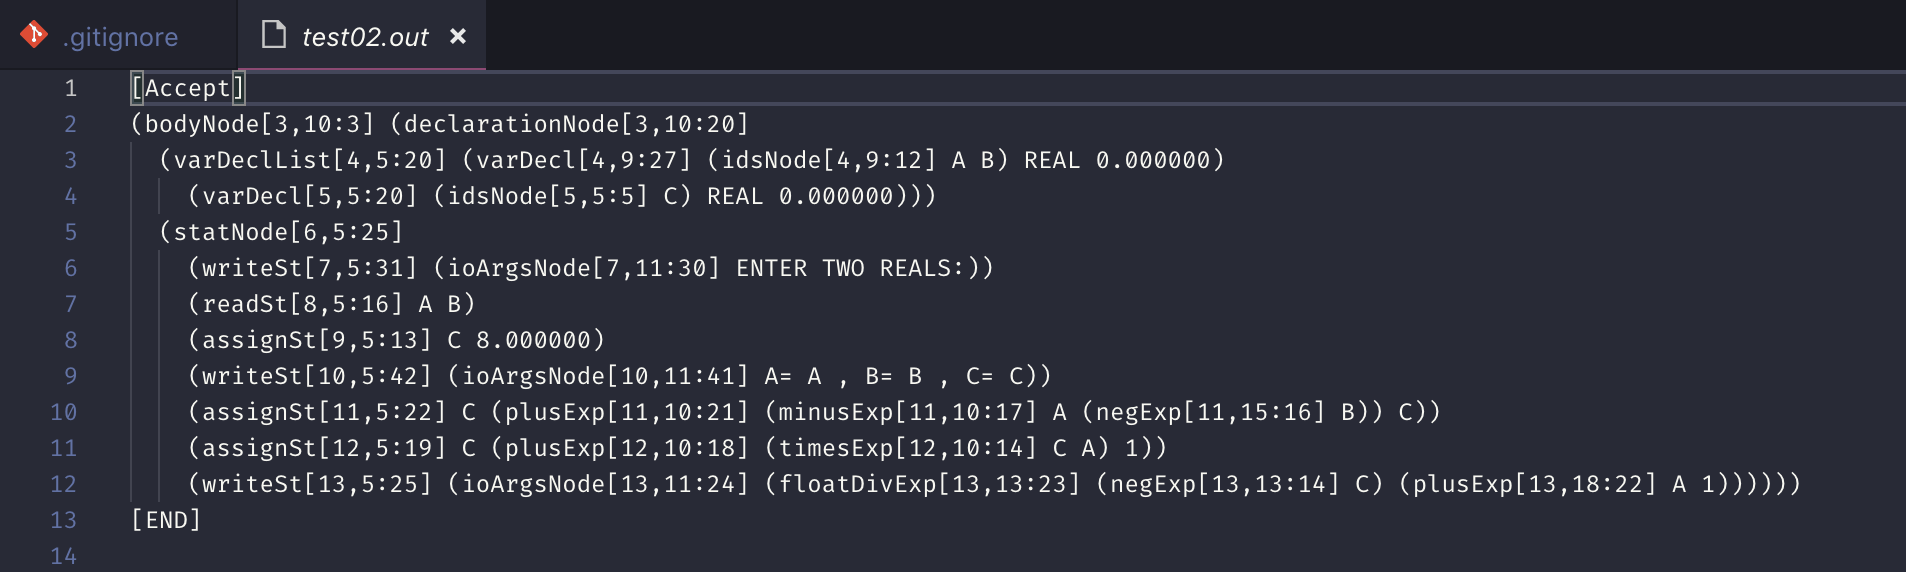
\includegraphics[width=0.7\linewidth]{correct}
		\caption{输出结果}
		\label{fig:correct}
	\end{figure}
	
	

\newpage
% File contents
\section{附录}

\subsection{EBNF}
\begin{footnotesize}
	\linespread{1.0}
	\lstinputlisting{../resource/syntax-ebnf.txt}
\end{footnotesize}


\newpage
\subsection{BNF}
\begin{footnotesize}
	\linespread{1.0}
	\lstinputlisting{../resource/syntax-bnf.txt}
\end{footnotesize}


\subsection{BNF-fixed}
\begin{footnotesize}
	\linespread{1.0}
	\lstinputlisting{../resource/syntax-bnf-fixed.txt}
\end{footnotesize}

\end{document}
